% This file is included by main.tex

\chapter{Wave Equation in 1D and 2D with Global Interpolation}
\label{ch::chapter8}

\section{Wave Equation 1D (Matrix–Vector)}
\label{sec:wave_1d_mxv}

\subsection{Mathematical model}

The one-dimensional wave equation can be expressed as:
\begin{equation}
\frac{\partial^2 u}{\partial t^2} = c^2 \frac{\partial^2 u}{\partial x^2}, 
\qquad x\in[0,L],\ t\ge 0,
\label{eq:wave_equation_1d}
\end{equation}

where $u(x,t)$ is the displacement at position $x$ and time $t$, and $c$ is the wave propagation speed. The initial condition and boundary conditions (homogeneous Dirichlet) are specified as:
\begin{align}
u(x,0) &= A\,\exp\!\left(-\frac{(x-x_c)^2}{2\sigma^2}\right), \qquad v(x,0) = 0,
\label{eq:initial_conditions_1d}
\end{align}
\vspace{-0.75em}
\begin{align}
u(0,t) = u(L,t) = 0, \qquad v(0,t) = v(L,t) = 0, \qquad t\ge 0.
\label{eq:boundary_conditions_1d}
\end{align}

where $A$ is the amplitude, $x_c$ is the center position, and $\sigma$ is the width of the initial Gaussian pulse, and $v(x,t) = \frac{\partial u}{\partial t}$ is the velocity field.

The wave equation can be reformulated as a first-order system by introducing the auxiliary variable $v(x,t) = \frac{\partial u}{\partial t}$:
\begin{equation}
\begin{aligned}
\frac{\partial u}{\partial t} &= v, \\
\frac{\partial v}{\partial t} &= c^2 \frac{\partial^2 u}{\partial x^2}.
\end{aligned}
\label{eq:coupled_system_1d}
\end{equation}

\subsubsection*{Spatial discretization (global interpolation)}
We discretize the spatial domain by selecting a set of collocation nodes
\(X=\{x_i\}_{i=0}^{N_x}\subset[0,L]\). The nodes may be uniform or nonuniform (e.g., Chebyshev–Lobatto).

The second derivative at the nodes is represented by the dense matrix \(\mathbf{D}_2^x\in\mathbb{R}^{(N_x+1)\times(N_x+1)}\) whose entries are the second derivatives of the basis functions evaluated at the nodes:
\begin{equation}
\mathbf{D}_2^x[i,j] \;=\; L_j''(x_i),\qquad i,j=0,\dots,N_x
\label{eq:D2x_def_wave}
\end{equation}

i.e., the global case of Eq.~\eqref{eq:D2_global_def}.

Given the nodal vector \(\mathbf{u}(t)=\big(u(x_0,t),\dots,u(x_{N_x},t)\big)^\top\),
the second derivative is approximated at the nodes by the matrix–vector product

\begin{equation}
u_{xx}(\cdot,t)\big|_{X}\;\approx\;\mathbf{D}_2^x\,\mathbf{u}(t).
\label{eq:u_xx_semidiscrete}
\end{equation}

\subsubsection*{Temporal discretization (explicit Euler)}
Writing the first–order system
\(
u_t=v,\quad v_t=c^2\,u_{xx}
\)
and inserting the semidiscrete operator \eqref{eq:u_xx_semidiscrete} gives the
ODE system for the nodal unknowns:
\begin{equation}
\frac{d\mathbf{u}}{dt} \;=\; \mathbf{v},\qquad
\frac{d\mathbf{v}}{dt} \;=\; c^2\,\mathbf{D}_2^x\,\mathbf{u}.
\label{eq:semi_discrete_ode}
\end{equation}

Collect the state at time level \(t^n\) as the stacked vector
\[
\mathbf{U}^{n}
=\begin{pmatrix}\mathbf{u}^{\,n}\\[0.25em]\mathbf{v}^{\,n}\end{pmatrix}
\in \mathbb{R}^{2(N_x+1)},
\qquad
\mathbf{F}^{n}
=\begin{pmatrix}\mathbf{v}^{\,n}\\[0.25em]c^2\,\mathbf{D}_2^x\,\mathbf{u}^{\,n}\end{pmatrix},
\]

so that a forward Euler step with time step \(\Delta t\) reads
\begin{equation}
\mathbf{U}^{\,n+1} \;=\; \mathbf{U}^{\,n} \;+\; \Delta t\,\mathbf{F}^{\,n}.
\label{eq:euler_update}
\end{equation}

This is followed immediately by the strong enforcement of the Dirichlet
constraints at the two boundary nodes for both \(u\) and \(v\).

The time step \(\Delta t\) must satisfy a CFL–like restriction to ensure stability of the explicit advance. This will be enforced by adjusting the time step based on the spatial grid size and wave speed.

\clearpage

\subsection{Code implementation}

The 1D wave solver stores the state in a rank-3 tensor \texttt{U} with shape
\((N_x\!+\!1,\ 2,\ N_t\!+\!1)\):
\begin{itemize}
  \item First dimension: spatial nodes \(x_i\), \(i=0,\dots,N_x\).
  \item Second dimension: fields (index 0 \(\to\) displacement \(u\), index 1 \(\to\) velocity \(v\)).
  \item Third dimension: time levels \(n=0,\dots,N_t\).
\end{itemize}

\noindent The Laplacian in 1D is applied by a single matrix–vector product with the
global second-derivative matrix \(\mathbf{D}_2^x\) from Eq.~\eqref{eq:D2x_def_wave}:
\begin{lstlisting}[language=Julia]
function laplacian_1D(U::OffsetArray{T}, D2x::OffsetArray{T}) where {T}
    return D2x * U[:, 0]
end
\end{lstlisting}
Here, \texttt{U[:, 0]} extracts the displacement vector \(\mathbf{u}^n\in\mathbb{R}^{N_x+1}\)
at the current time step, and \texttt{D2x * U[:, 0]} returns an approximation of
\(\partial^2 u/\partial x^2\) at all nodes (cf. Eq.~\eqref{eq:D2x_def_wave}).

\medskip
\noindent The explicit Euler advance follows the block form in
Eq.~\eqref{eq:euler_update}:
\begin{lstlisting}[language=Julia]
apply_dirichlet!(U, n, Nx)           # enforce homogeneous BCs at t^n
L = laplacian_1D(U[:, :, n], D2x) 

@views begin
    F[:, 0] .= U[:, 1, n]              # RHS for u_t = v
    F[:, 1] .= c^2 .* L                # RHS for v_t = c^2 u_xx
    U[:, :, n+1] .= U[:, :, n] .+ dt .* F
end

apply_dirichlet!(U, n+1, Nx)           # enforce BCs at t^(n+1)
\end{lstlisting}

The working array \texttt{F} has shape \((N_x\!+\!1,2)\) and stores the right-hand
side \(\big[\mathbf{v}^n,\ c^2\mathbf{D}_2^x\mathbf{u}^n\big]\).
Boundary conditions are imposed strongly by overwriting the boundary
entries of \(u\) and \(v\) at each step.

The differentiation matrix \(\mathbf{D}_2^x\) is built once, at startup, via the
global Lagrange construction, choosing a stencil size of \(N_x+1\):
\begin{lstlisting}[language=Julia]
D2x = OffsetArray(build_D2_matrix(xnodes, stencil, T), 0:Nx, 0:Nx)
\end{lstlisting}
Here \texttt{xnodes} holds the collocation nodes (uniform or nonuniform, e.g.,
Chebyshev–Lobatto). With \texttt{stencil\_size = Nx+1} the operator is global
and therefore dense; smaller stencils would yield a banded \(\mathbf{D}_2^x\).
The dominant kernel per step is the BLAS \texttt{gemv} \(\mathbf{D}_2^x\mathbf{u}^n\).

\clearpage

\subsection{Results}

\subsubsection*{Laplacian Operator FP32 Performance}

The isolated 1D Laplacian operator performance demonstrates characteristic memory-bound behavior, consistent with the matrix-vector benchmarks analyzed in Chapter 3.

\vspace{-0.5em}

\begin{figure}[H]\centering
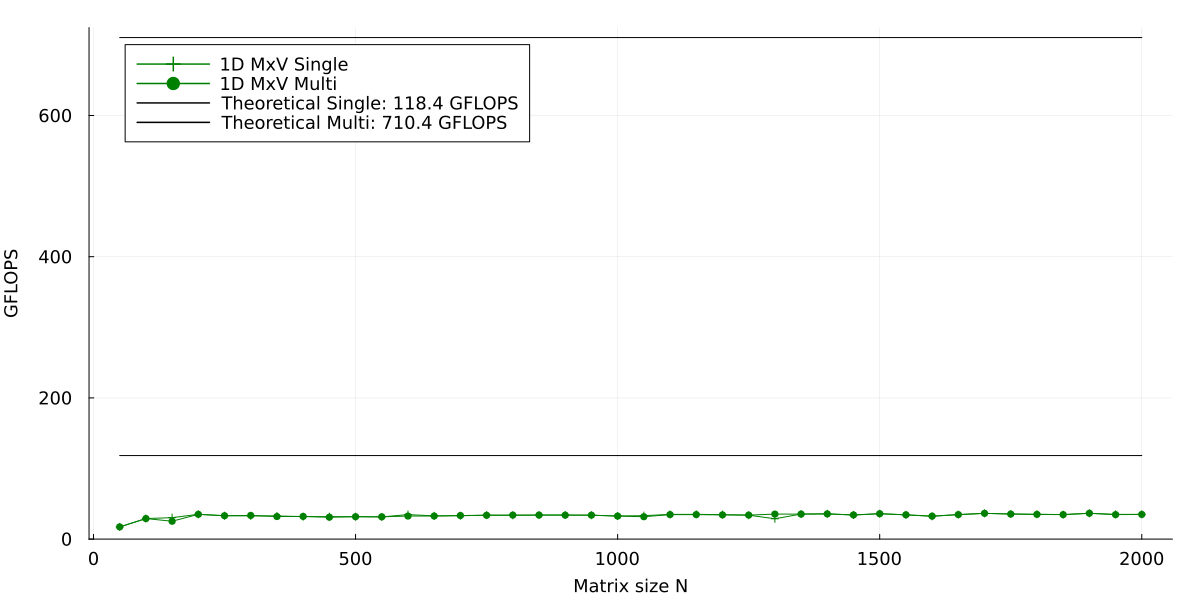
\includegraphics[width=\textwidth]{figures/8_wave_equation_solvers/Float32_GFLOPS_laplacian_1D_MxV.png}
\caption{\textbf{Float32 1D Laplacian (MxV): single vs. multi-threaded performance.} Single-threaded performance shows steady, memory-bound behavior with gradual improvement. Multi-threaded performance closely matches single-threaded initially but exhibits dramatic degradation around mid-range sizes before recovering at larger scales.}
\end{figure}

\textbf{Memory-bound plateau behavior}: Both curves plateau well below compute-bound performance levels, reflecting the low arithmetic intensity inherent to matrix-vector operations. This behavior mirrors the synthetic MxV benchmarks from Chapter 3, where memory bandwidth becomes the fundamental bottleneck regardless of computational resources.

% \textbf{Threading penalty phenomenon}: The sharp multi-threaded performance drop at intermediate sizes demonstrates cache contention effects absent in synthetic benchmarks. Multiple threads competing for the same memory subsystem create bottlenecks that actually reduce performance below single-threaded levels.

\textbf{Consistent single-threaded efficiency}: The stable single-threaded curve across all sizes confirms that memory bandwidth limitation dominates performance, avoiding the complications of inter-thread resource competition.

This 1D implementation validates the theoretical predictions from Chapter 3 regarding matrix-vector limitations, demonstrating that real-world PDE operators exhibit the same fundamental memory-bound characteristics as synthetic benchmarks.

\clearpage

\subsubsection*{1D Wave Equation (MxV) FP64 Performance}

We evaluated the complete 1D wave equation solver across a range of grid sizes using \textbf{Float64 precision} and 1.0 second simulation time. 

Each time step involves matrix-vector multiplication, plus additional operations for temporal integration and boundary condition enforcement. The total floating-point operations per time step can be approximated as \(2 \times N_x^2\) (dominated by the MxV operation):

\begin{equation}
\text{Total Operations} =  \text{Time Steps} \times \text{Operations per Step} \approx N_t \times 2 \times N_x^2
\end{equation}

We used an adaptive time step of $dt = 10^{-4} \times \frac{1}{N_{x}}$ seconds for stability control. This formulation ensures that finer grids use proportionally smaller time steps.

\vspace{1em}


\begin{tabular*}{\linewidth}{@{\extracolsep{\fill}}cccc}
\toprule
\textbf{Grid Size} & \textbf{Time (s)} & \textbf{Total Operations} & \textbf{GFLOPS} \\
\midrule
26 nodes  & 0.10 & 3.52 $\times$ 10$^{8}$  & 3.52 \\
51 nodes  & 0.35 & 2.65 $\times$ 10$^{9}$  & 7.58 \\
76 nodes  & 0.90 & 8.78 $\times$ 10$^{9}$  & 9.76 \\
101 nodes & 1.95 & 2.06 $\times$ 10$^{10}$ & 10.57 \\
126 nodes & 3.66 & 4.00 $\times$ 10$^{10}$ & 10.93 \\
151 nodes & 6.05 & 6.89 $\times$ 10$^{10}$ & 11.38 \\
176 nodes & 8.91 & 1.09 $\times$ 10$^{11}$ & 12.24 \\
201 nodes & 13.47 & 1.62 $\times$ 10$^{11}$ & 12.06 \\
\bottomrule
\end{tabular*}

\vspace{1em}

The performance progression shows consistent scaling behavior across all grid sizes. For small grids (26-76 nodes), we observe steady efficiency improvements as matrix operations begin to dominate computational overhead. The medium grids (101-151 nodes) show continued linear scaling reaching peak efficiency around 11.3 GFLOPS. Finally, large grids (176-201 nodes) exhibit a performance plateau near 12.1 GFLOPS, indicating optimal throughput for this precision.

These results align closely with the Float64 matrix-vector multiplication performance characteristics observed in Chapter 3, confirming that the wave equation solver achieves the expected computational efficiency for dense linear algebra operations. The final performance of approximately 12 GFLOPS demonstrates that the full solver maintains the same computational characteristics as the isolated matrix-vector benchmarks.

\clearpage

\textbf{Physical 1D Wave Evolution (MxV) - Original Nodes Representation}

The solver captures correct wave physics across all stable configurations. Using N=25 nodes with 26-node stencil demonstrates complete wave propagation behavior:

\vspace{0.5em}

\begin{figure}[H]
\centering
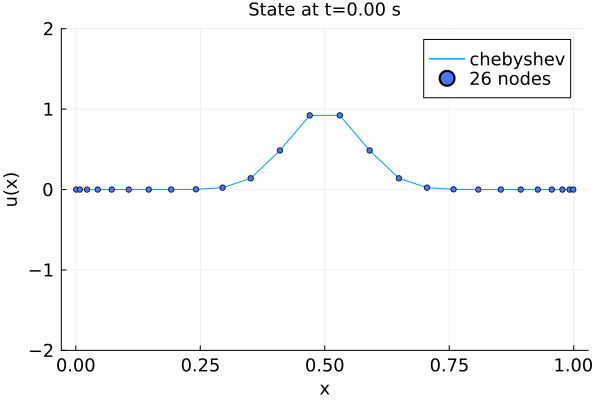
\includegraphics[width=0.48\textwidth]{code/8_wave_equation_solvers/benchmark_versions/output/output1D_25_benchmark/state_t_0.00.png}
\hfill
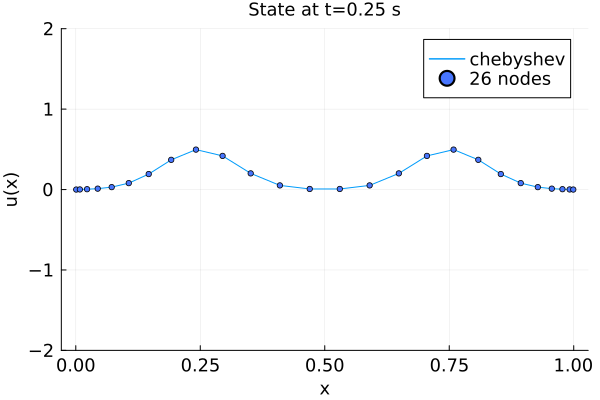
\includegraphics[width=0.48\textwidth]{code/8_wave_equation_solvers/benchmark_versions/output/output1D_25_benchmark/state_t_0.25.png}

\vspace{1em}

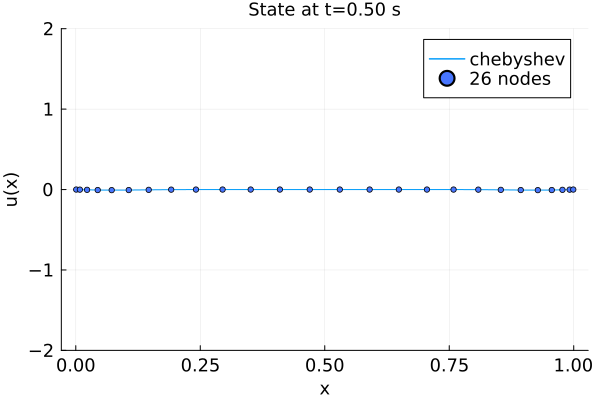
\includegraphics[width=0.48\textwidth]{code/8_wave_equation_solvers/benchmark_versions/output/output1D_25_benchmark/state_t_0.50.png}
\hfill
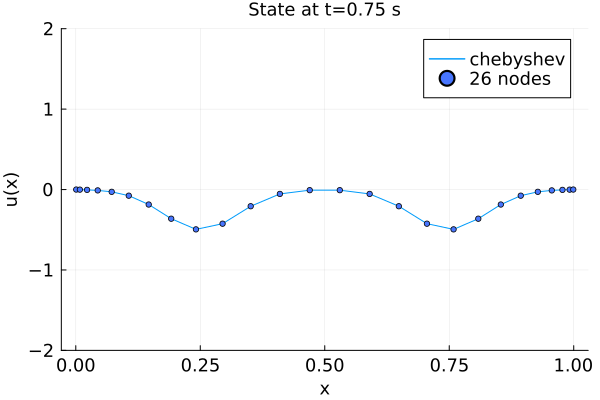
\includegraphics[width=0.48\textwidth]{code/8_wave_equation_solvers/benchmark_versions/output/output1D_25_benchmark/state_t_0.75.png}

\vspace{1em}

\centering
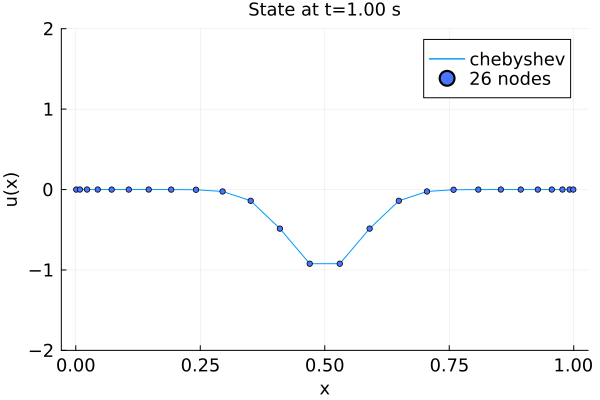
\includegraphics[width=0.48\textwidth]{code/8_wave_equation_solvers/benchmark_versions/output/output1D_25_benchmark/state_t_1.00.png}

\caption{\textbf{1D Wave Equation Evolution.} The temporal sequence shows: (top left) initial Gaussian pulse centered at x = 0.5, (top right) wave splitting into counter-propagating components, (middle left) reflection at Dirichlet boundaries, (middle right) wave interference during convergence, and (bottom) final standing wave configuration. Blue circles indicate the 26 Chebyshev node positions where the discrete solution is computed.}
\end{figure}

\clearpage

\textbf{Physical 1D Wave Evolution (MxV) - Interpolated Representation}

The Chebyshev node distribution enables high-quality Lagrange interpolation to reconstruct the continuous wave field. The solution is interpolated from 26 Chebyshev nodes to 100 equispaced points:

\vspace{0.5em}

\begin{figure}[H]
\centering
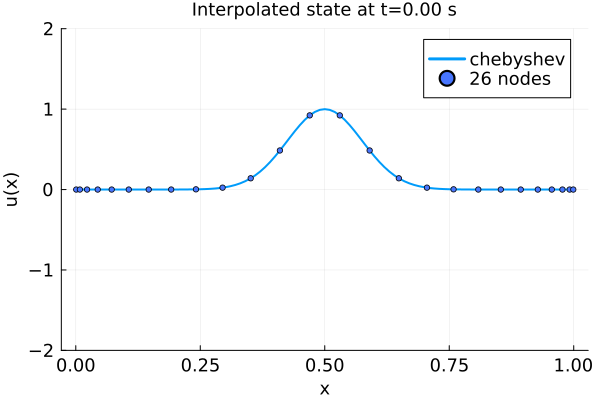
\includegraphics[width=0.48\textwidth]{code/8_wave_equation_solvers/benchmark_versions/output/output1D_25_benchmark/interpolated_state_t_0.00.png}
\hfill
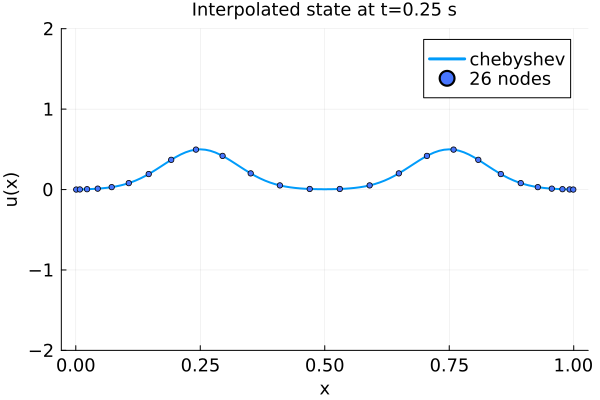
\includegraphics[width=0.48\textwidth]{code/8_wave_equation_solvers/benchmark_versions/output/output1D_25_benchmark/interpolated_state_t_0.25.png}

\vspace{1em}

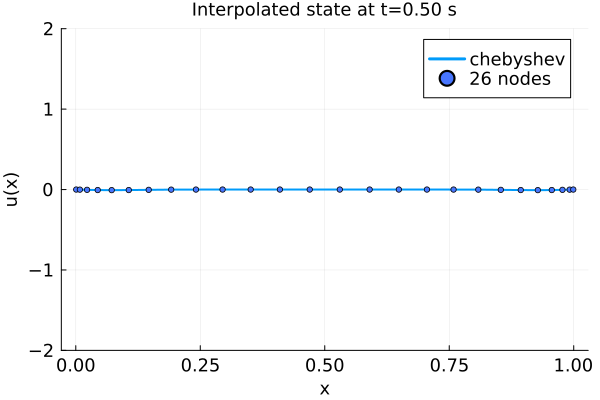
\includegraphics[width=0.48\textwidth]{code/8_wave_equation_solvers/benchmark_versions/output/output1D_25_benchmark/interpolated_state_t_0.50.png}
\hfill
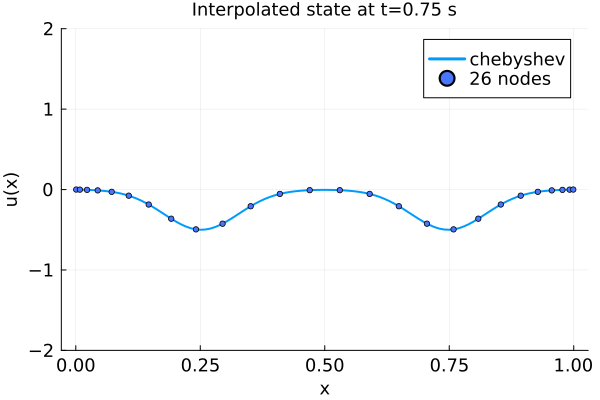
\includegraphics[width=0.48\textwidth]{code/8_wave_equation_solvers/benchmark_versions/output/output1D_25_benchmark/interpolated_state_t_0.75.png}

\vspace{1em}

\centering
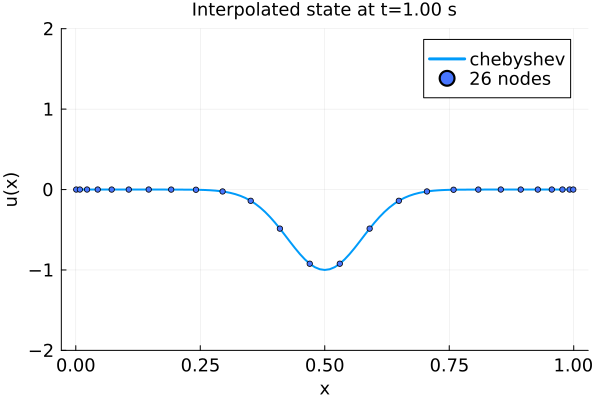
\includegraphics[width=0.48\textwidth]{code/8_wave_equation_solvers/benchmark_versions/output/output1D_25_benchmark/interpolated_state_t_1.00.png}

\caption{\textbf{1D Wave Equation Evolution (Fine Grid).} The continuous curves demonstrate the high accuracy of Lagrange interpolation from the optimal Chebyshev node distribution (blue circles) to a fine equispaced grid of 100 points.}
\end{figure}

\clearpage

\section{Wave Equation 2D (Matrix–Matrix)}
\label{sec:wave_2d_mxm}

\subsection{Mathematical model}

The two-dimensional wave equation can be expressed as:
\begin{equation}
\frac{\partial^2 u}{\partial t^2} = c^2 \left(\frac{\partial^2 u}{\partial x^2} + \frac{\partial^2 u}{\partial y^2}\right), 
\qquad (x,y)\in[0,L_x]\times[0,L_y],\ t\ge 0,
\label{eq:wave_equation_2d}
\end{equation}

where $u(x,y,t)$ is the displacement at position $(x,y)$ and time $t$, and $c$ is the wave propagation speed. The initial condition and boundary conditions (homogeneous Dirichlet) are specified as:
\begin{align}
u(x,y,0) &= A\,\exp\!\left(-\frac{(x-x_c)^2+(y-y_c)^2}{2\sigma^2}\right), \qquad v(x,y,0) = 0,
\label{eq:initial_conditions_2d}
\end{align}
\vspace{-0.75em}
\begin{align}
u(0,y,t) = u(L_x,y,t) = u(x,0,t) = u(x,L_y,t) = 0, \hspace{4.7em}\\
v(0,y,t) = v(L_x,y,t) = v(x,0,t) = v(x,L_y,t) = 0, \qquad t\ge 0.
\label{eq:boundary_conditions_2d}
\end{align}

where $A$ is the amplitude, $(x_c,y_c)$ is the center position, and $\sigma$ is the width of the initial Gaussian pulse, and $v(x,y,t) = \frac{\partial u}{\partial t}$ is the velocity field.

The wave equation can be reformulated as a first-order system by introducing the auxiliary variable $v(x,y,t) = \frac{\partial u}{\partial t}$:
\begin{equation}
\begin{aligned}
\frac{\partial u}{\partial t} &= v, \\
\frac{\partial v}{\partial t} &= c^2 \left(\frac{\partial^2 u}{\partial x^2} + \frac{\partial^2 u}{\partial y^2}\right).
\end{aligned}
\label{eq:coupled_system_2d}
\end{equation}

\subsubsection*{Spatial discretization (global interpolation)}

We discretize the spatial domain using a tensor-product grid by selecting collocation nodes
$X^{(x)}=\{x_i\}_{i=0}^{N_x}\subset[0,L_x]$ and $X^{(y)}=\{y_j\}_{j=0}^{N_y}\subset[0,L_y]$. The nodes may be uniform or nonuniform (e.g., Chebyshev–Lobatto) in each direction.

The 2D Laplacian at grid point $(x_i,y_j)$ splits additively: $\nabla^2 u(x_i,y_j) = u_{xx}(x_i,y_j) + u_{yy}(x_i,y_j)$.

The directional second derivatives are represented by dense matrices $\mathbf{D}_2^x\in\mathbb{R}^{(N_x+1)\times(N_x+1)}$ and $\mathbf{D}_2^y\in\mathbb{R}^{(N_y+1)\times(N_y+1)}$ whose entries are the second derivatives of the basis functions evaluated at the nodes:
\begin{align}
\mathbf{D}_2^x[i,k] &= L_k^{(x)\prime\prime}(x_i),\qquad i,k=0,\dots,N_x \\
\mathbf{D}_2^y[j,\ell] &= L_\ell^{(y)\prime\prime}(y_j),\qquad j,\ell=0,\dots,N_y
\label{eq:D2xy_def_wave}
\end{align}

i.e., the global case of Eq.~\eqref{eq:D2_global_def} applied in each direction.

\clearpage

Given the displacement field as a matrix $\mathbf{U}(t)\in\mathbb{R}^{(N_x+1)\times(N_y+1)}$ with $\mathbf{U}[i,j](t) = u(x_i,y_j,t)$, where rows correspond to different $x_i$ values and columns to different $y_j$ values, the directional derivatives are computed as:
\begin{align}
u_{xx}(\cdot,\cdot,t) &\approx \mathbf{D}_2^x\,\mathbf{U}(t) \qquad \text{(acts on each column, fixed $y_j$)} \\
u_{yy}(\cdot,\cdot,t) &\approx \mathbf{U}(t)\,(\mathbf{D}_2^y)^\top \qquad \text{(acts on each row, fixed $x_i$)}
\end{align}

The transpose in the $y$-derivative appears because $\mathbf{D}_2^y$ is designed to act on column vectors of $y$-direction values, but we need to apply it to each row of $\mathbf{U}$ (corresponding to fixed $x_i$). The matrix multiplication $\mathbf{U}\,(\mathbf{D}_2^y)^\top$ is equivalent to applying $\mathbf{D}_2^y$ to each row vector $\mathbf{U}[i,:]$ and can be understood as:
\[
\big(\mathbf{U}\,(\mathbf{D}_2^y)^\top\big)[i,j] = \sum_{\ell=0}^{N_y} \mathbf{U}[i,\ell] \, (\mathbf{D}_2^y)^\top[\ell,j] = \sum_{\ell=0}^{N_y} \mathbf{D}_2^y[j,\ell] \, u(x_i,y_\ell)
\]
which correctly computes the $y$-derivative at $(x_i,y_j)$ using values along the fixed $x_i$ line.

The 2D Laplacian is then approximated by:
\begin{equation}
\nabla^2 u(\cdot,\cdot,t)\big|_{X^{(x)}\times X^{(y)}}\;\approx\;\mathbf{D}_2^x\,\mathbf{U}(t) + \mathbf{U}(t)\,(\mathbf{D}_2^y)^\top.
\label{eq:laplacian_2d_semidiscrete}
\end{equation}

\subsubsection*{Temporal discretization (explicit Euler)}

Writing the first–order system
$u_t=v$, $v_t=c^2\,(\,u_{xx}+u_{yy})$
and inserting the semidiscrete operator \eqref{eq:laplacian_2d_semidiscrete} gives the
ODE system for the nodal unknowns:
\begin{equation}
\frac{d\mathbf{U}}{dt} \;=\; \mathbf{V},\qquad
\frac{d\mathbf{V}}{dt} \;=\; c^2\,\left(\mathbf{D}_2^x\,\mathbf{U} + \mathbf{U}\,(\mathbf{D}_2^y)^\top\right).
\label{eq:semi_discrete_ode_2d}
\end{equation}

Collect the state at time level $t^n$ as the stacked tensor
\[
\mathbf{U}^{\,n}
=\begin{pmatrix}\mathbf{u}^{\,n}\\\mathbf{v}^{\,n}\end{pmatrix}
\in \mathbb{R}^{(N_x+1)\times(N_y+1)\times 2},
\qquad
\mathbf{F}^{\,n}
=\begin{pmatrix}\mathbf{v}^{\,n}\\c^2\,\left(\mathbf{D}_2^x\,\mathbf{u}^{\,n} + \mathbf{u}^{\,n}\,(\mathbf{D}_2^y)^\top\right)\end{pmatrix},
\]
so that a forward Euler step with time step $\Delta t$ reads
\begin{equation}
\mathbf{U}^{\,n+1} \;=\; \mathbf{U}^{\,n} \;+\; \Delta t\,\mathbf{F}^{\,n}.
\label{eq:euler_update_2d}
\end{equation}

This is followed immediately by the strong enforcement of the Dirichlet
constraints at all four boundary edges for both $u$ and $v$.

In 2D, the choice of $\Delta t$ must satisfy a CFL–like restriction governed by the
smallest grid spacing in both directions, which ensures stability of the explicit advance.

\clearpage

\subsection{Code implementation}

The 2D wave solver stores the state in a rank-4 tensor \texttt{U} with shape
$(N_x\!+\!1,\ N_y\!+\!1,\ 2,\ N_t\!+\!1)$:
\begin{itemize}
  \item First dimension: spatial nodes $x_i$, $i=0,\dots,N_x$.
  \item Second dimension: spatial nodes $y_j$, $j=0,\dots,N_y$.
  \item Third dimension: fields (index 0 $\to$ displacement $u$, index 1 $\to$ velocity $v$).
  \item Fourth dimension: time levels $n=0,\dots,N_t$.
\end{itemize}

\noindent The Laplacian in 2D is applied by two matrix–matrix products with the
global second-derivative matrices $\mathbf{D}_2^x$ and $\mathbf{D}_2^y$ from Eq.~\eqref{eq:D2xy_def_wave}:
\begin{lstlisting}[language=Julia]
function laplacian_2D(U::OffsetArray{T}, D2x::OffsetArray{T}, D2yT::OffsetArray{T}) where {T}
    return D2x * U[:, :, 0] .+ U[:, :, 0] * D2yT
end
\end{lstlisting}
Here, \texttt{U[:, :, 0]} extracts the displacement matrix $\mathbf{u}^n\in\mathbb{R}^{(N_x+1)\times(N_y+1)}$
at the current time step. The operation \texttt{D2x * U[:, :, 0]} applies the x-direction second derivative to each column (fixed $y_j$), while \texttt{U[:, :, 0] * D2yT} applies the y-direction second derivative to each row (fixed $x_i$), returning approximations of $\partial^2 u/\partial x^2$ and $\partial^2 u/\partial y^2$ respectively (cf. Eq.~\eqref{eq:laplacian_2d_semidiscrete}).

\medskip
\noindent The explicit Euler advance follows the block form in
Eq.~\eqref{eq:euler_update_2d}:
\begin{lstlisting}[language=Julia]
apply_dirichlet!(U, n, Nx, Ny)           # enforce homogeneous BCs at t^n
L = laplacian_2D(U[:, :, :, n], D2x, D2yT) 

@views begin
    F[:, :, 0] .= U[:, :, 1, n]           # RHS for u_t = v
    F[:, :, 1] .= c^2 .* L                # RHS for v_t = c^2 (u_xx + u_yy)
    U[:, :, :, n+1] .= U[:, :, :, n] .+ dt .* F
end

apply_dirichlet!(U, n+1, Nx, Ny)         # enforce BCs at t^(n+1)
\end{lstlisting}

The working array \texttt{F} has shape $(N_x\!+\!1,N_y\!+\!1,2)$ and stores $\big[\mathbf{v}^n,\ c^2(\mathbf{D}_2^x\mathbf{u}^n + \mathbf{u}^n(\mathbf{D}_2^y)^\top)\big]$.
Boundary conditions are imposed strongly by overwriting the boundary
entries of $u$ and $v$ at each step on all four edges.

The differentiation matrices $\mathbf{D}_2^x$ and $\mathbf{D}_2^y$ are built once, at startup, via the
global Lagrange construction, choosing stencil sizes of $N_x+1$ and $N_y+1$ respectively:
\begin{lstlisting}[language=Julia]
D2x = OffsetArray(build_D2_matrix(xnodes, Nx+1, T), 0:Nx, 0:Nx)
D2y = OffsetArray(build_D2_matrix(ynodes, Ny+1, T), 0:Ny, 0:Ny)
D2yT = transpose(D2y)
\end{lstlisting}
Here \texttt{xnodes} and \texttt{ynodes} hold the collocation nodes in each direction (uniform or nonuniform, e.g.,
Chebyshev–Lobatto). With \texttt{stencil\_size = Nx+1} and \texttt{Ny+1} the operators are global
and therefore dense; smaller stencils would yield banded matrices.
The dominant kernels per step are the two BLAS \texttt{gemm} operations $\mathbf{D}_2^x\mathbf{u}^n$ and $\mathbf{u}^n(\mathbf{D}_2^y)^\top$.

\clearpage

\subsection{Results}

\subsubsection*{Laplacian Operator FP32 Performance}

The 2D matrix-matrix Laplacian operator demonstrates exceptional computational efficiency, exhibiting behavior consistent with the synthetic benchmarks from Chapter 3.

\vspace{-0.5em}

\begin{figure}[H]\centering
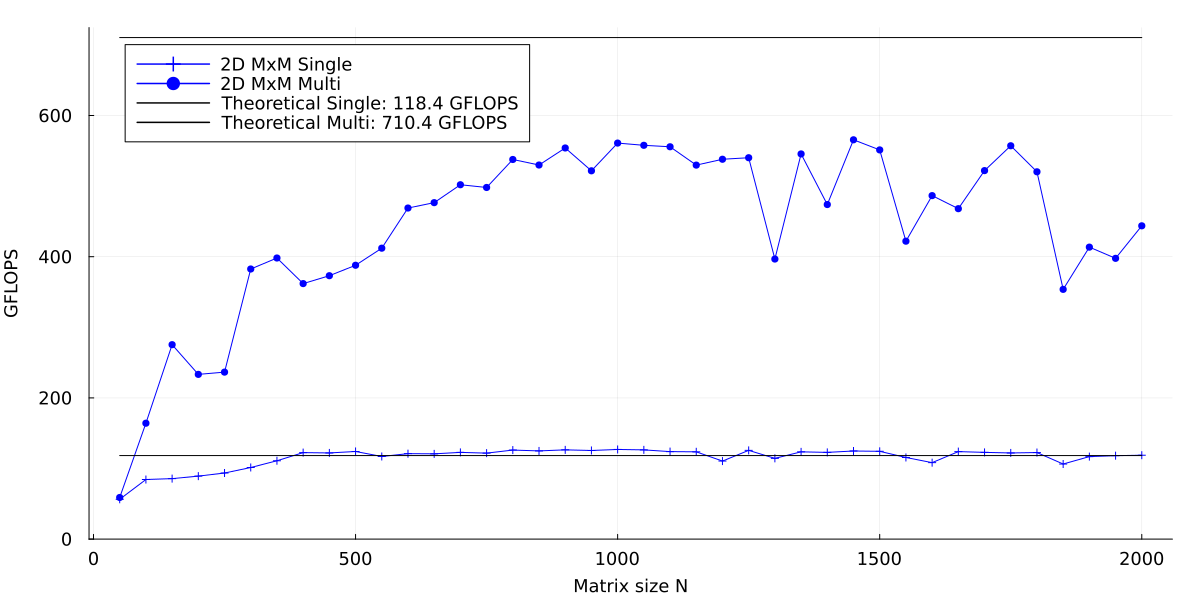
\includegraphics[width=\textwidth]{figures/8_wave_equation_solvers/Float32_GFLOPS_laplacian_2D_MxM.png}
\caption{\textbf{Float32 2D Laplacian (MxM): single vs. multi-threaded performance.} Single-threaded performance steadily improves with matrix size, achieving theoretical performance due to turbo boost effects. Multi-threaded performance shows dramatic scaling with a sharp transition, though remaining below theoretical peaks due to shared resource contention.}
\end{figure}

\textbf{Single-threaded theoretical convergence}: The single-threaded curve reaches and slightly exceeds theoretical performance, mirroring Chapter 3 results. This reflects turbo boost effects where single-core workloads benefit from higher frequencies than base clock calculations assume.

\textbf{Multi-threaded scaling limitations}: Multi-threaded performance exhibits the characteristic sharp transition seen in synthetic benchmarks but remains below theoretical peaks. This gap reflects shared resource contention (L3 cache, memory bandwidth) and lower all-core turbo frequencies, consistent with our earlier analysis.

\textbf{BLAS optimization effectiveness}: The two matrix-matrix products ($\mathbf{D}_2^x\mathbf{u}$ and $\mathbf{u}(\mathbf{D}_2^y)^\top$) achieve compute-bound performance through optimized \texttt{gemm} kernels, demonstrating superior arithmetic intensity compared to matrix-vector alternatives.

The close correspondence with Chapter \ref{ch::chapter3} synthetic results confirms that real-world PDE solvers can achieve predicted computational efficiency when algorithmic structure aligns with modern CPU architectures.

\clearpage

\subsubsection*{2D Wave Equation (MxM) FP64 Performance}

We evaluated the complete 2D wave equation solver across a range of grid sizes using \textbf{Float64 precision} and 1.0 second simulation time.

Each time step involves matrix-matrix multiplication operations, plus additional operations for temporal integration and boundary condition enforcement. The total floating-point operations per time step can be approximated as $2 \times 2 \times N^3$ (dominated by the MxM operations):

\begin{equation}
\text{Total Operations} = \text{Time Steps} \times \text{Operations per Step} \approx N_t \times 2 \times 2 \times N^3
\end{equation}

We used an adaptive time step of $dt = 10^{-4} \times \frac{1}{N_{x}}$ seconds for stability control. This formulation ensures that finer grids use proportionally smaller time steps.

\vspace{0.5em}

\begin{table}[ht]
\centering
\begin{tabular*}{\linewidth}{@{\extracolsep{\fill}}cccc}
\toprule
\textbf{Grid Size} & \textbf{Time (s)} & \textbf{Total Operations} & \textbf{GFLOPS} \\
\midrule
26 nodes  & 6.50   & 1.83 $\times$ 10$^{10}$ & 2.81 \\
51 nodes  & 22.12  & 2.71 $\times$ 10$^{11}$ & 12.23 \\
76 nodes  & 58.44  & 1.33 $\times$ 10$^{12}$ & 22.84 \\
101 nodes & 118.34 & 4.16 $\times$ 10$^{12}$ & 35.17 \\
126 nodes & 207.86 & 1.01 $\times$ 10$^{13}$ & 48.50 \\
151 nodes & 398.64 & 2.08 $\times$ 10$^{13}$ & 52.17 \\
176 nodes & 546.00 & 3.84 $\times$ 10$^{13}$ & 70.29 \\
201 nodes & 919.12 & 6.53 $\times$ 10$^{13}$ & 71.03 \\
\bottomrule
\end{tabular*}
\end{table}


\vspace{1em}

The performance progression demonstrates a scaling behavior across all grid sizes. For small grids (26-76 nodes), we observe rapid efficiency improvements as the cubic scaling of matrix operations begins to dominate computational overhead. The medium grids (101-151 nodes) show continued strong scaling with performance reaching over 50 GFLOPS. Finally, large grids (176-201 nodes) exhibit peak performance near 70 GFLOPS.

This demonstrates the superior computational characteristics of 2D matrix-matrix operations compared to 1D matrix-vector operations. The cubic scaling of operations with grid size ($N^3$) enables higher arithmetic intensity, leading to significantly better GFLOPS performance.

We observe that the performance is still below of what was achieved in the synthetic benchmarks in Chapter 3, likely due to the additional overhead of boundary condition enforcement and temporal integration steps that are not present in isolated matrix-matrix multiplication tests.

\clearpage

\textbf{Physical 2D Wave Evolution (MxM) - Original Nodes Representation}

The 2D solver captures complete wave physics on Chebyshev node grids. Using 25×25 nodes with 26-node stencils demonstrates radial wave propagation and boundary interactions:

\begin{figure}[H]
\centering
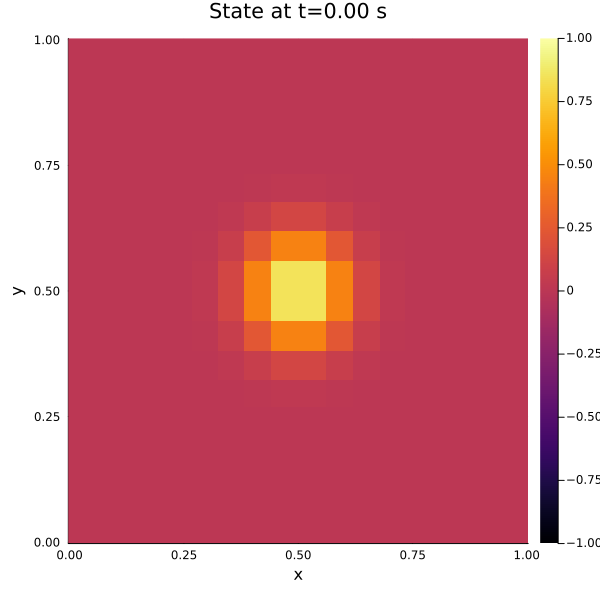
\includegraphics[width=0.48\textwidth]{code/8_wave_equation_solvers/benchmark_versions/output/output2D_25_MxM_benchmark/state_t_0.00.png}
\hfill
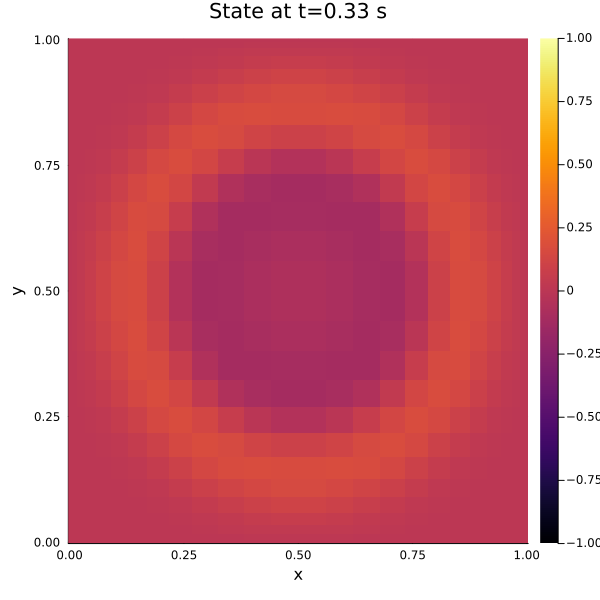
\includegraphics[width=0.48\textwidth]{code/8_wave_equation_solvers/benchmark_versions/output/output2D_25_MxM_benchmark/state_t_0.33.png}

\vspace{1em}

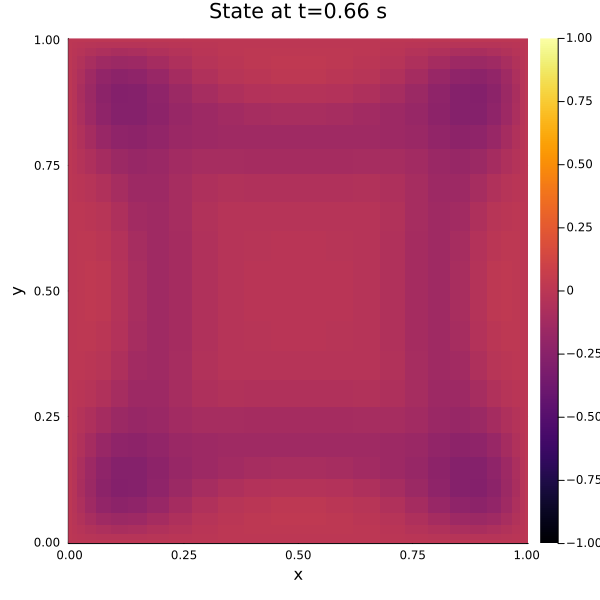
\includegraphics[width=0.48\textwidth]{code/8_wave_equation_solvers/benchmark_versions/output/output2D_25_MxM_benchmark/state_t_0.66.png}
\hfill
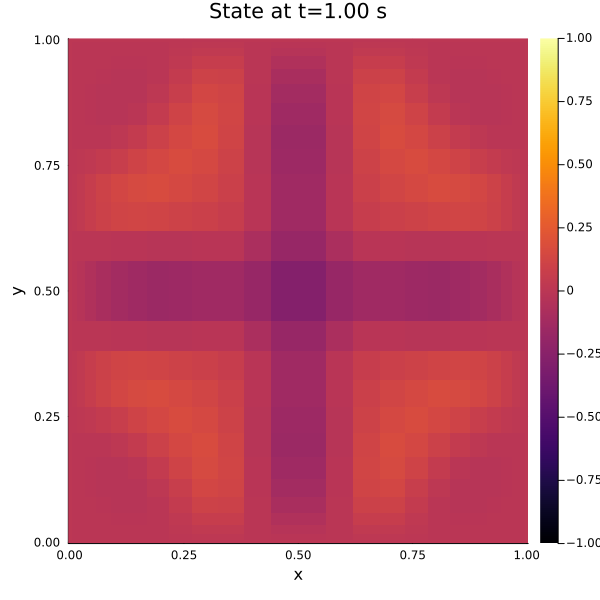
\includegraphics[width=0.48\textwidth]{code/8_wave_equation_solvers/benchmark_versions/output/output2D_25_MxM_benchmark/state_t_1.00.png}

\caption{\textbf{2D Wave Equation Evolution.} The temporal sequence shows: (top left) initial Gaussian pulse centered at domain center, (top right) radial wave expansion at t=0.33s, (bottom left) complex interference patterns at t=0.66s, and (bottom right) final standing wave configuration with multiple nodes at t=1.0s. The discrete solution is computed on a 26×26 Chebyshev node grid.}
\end{figure}

\clearpage

\textbf{Physical 2D Wave Evolution (MxM) - Interpolated Representation}

The 2D Chebyshev node distribution enables high-quality tensor-product Lagrange interpolation to reconstruct the continuous wave field. The solution is interpolated from 26×26 Chebyshev nodes to a 100×100 equispaced grid:

\begin{figure}[H]
\centering
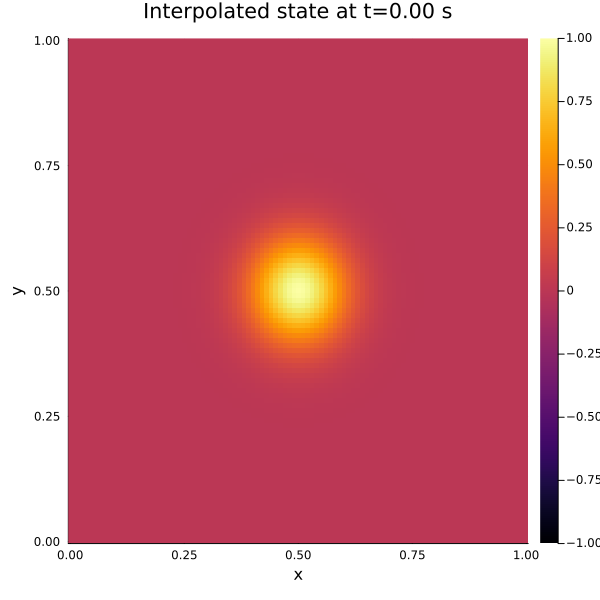
\includegraphics[width=0.48\textwidth]{code/8_wave_equation_solvers/benchmark_versions/output/output2D_25_MxM_benchmark/interpolated_state_t_0.00.png}
\hfill
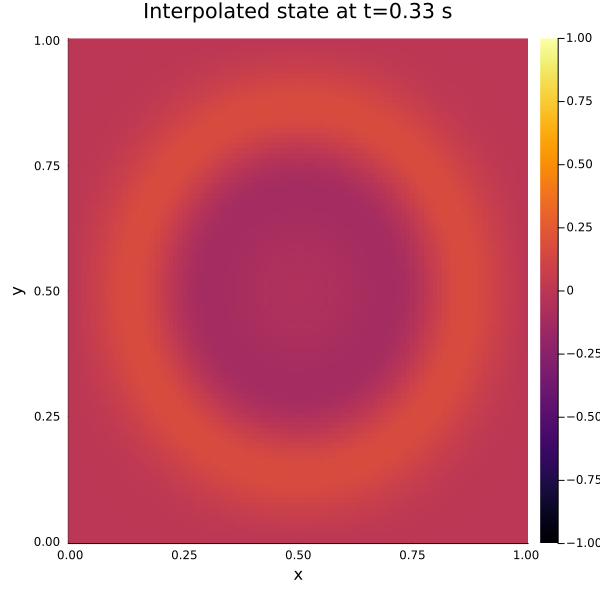
\includegraphics[width=0.48\textwidth]{code/8_wave_equation_solvers/benchmark_versions/output/output2D_25_MxM_benchmark/interpolated_state_t_0.33.png}

\vspace{1em}

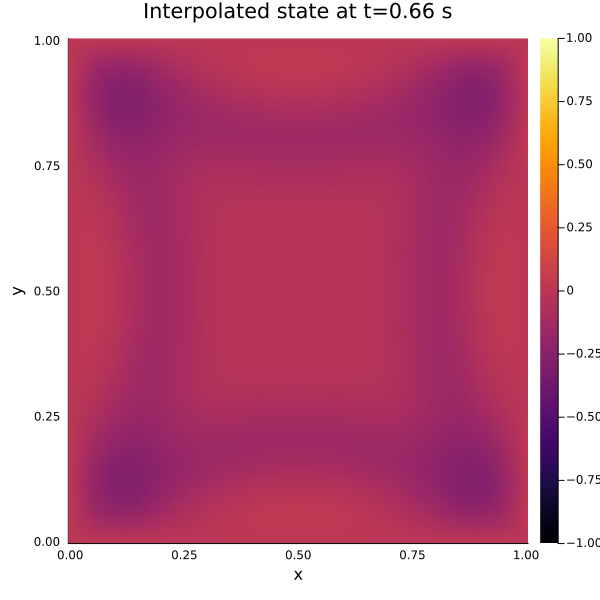
\includegraphics[width=0.48\textwidth]{code/8_wave_equation_solvers/benchmark_versions/output/output2D_25_MxM_benchmark/interpolated_state_t_0.66.png}
\hfill
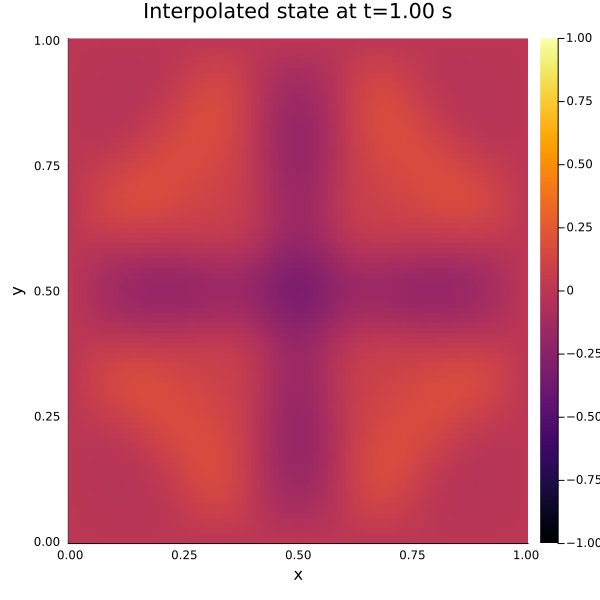
\includegraphics[width=0.48\textwidth]{code/8_wave_equation_solvers/benchmark_versions/output/output2D_25_MxM_benchmark/interpolated_state_t_1.00.png}

\caption{\textbf{2D Wave Equation Evolution. (Fine Grid)} The smooth contours demonstrate excellent interpolation accuracy from the optimal 26×26 Chebyshev node distribution to a fine 100×100 equispaced visualization grid. The tensor-product interpolation preserves wave symmetry and captures fine-scale interference patterns throughout the temporal evolution.}
\end{figure}

\clearpage

\section{Wave Equation 2D (Looped Matrix–Vector)}
\label{sec:wave_2d_mxv}

\subsection{Mathematical model}

The mathematical formulation is identical to Section~\ref{sec:wave_2d_mxm}, solving the 2D wave equation:
\begin{equation}
\frac{\partial^2 u}{\partial t^2} = c^2 \left(\frac{\partial^2 u}{\partial x^2} + \frac{\partial^2 u}{\partial y^2}\right),
\qquad (x,y)\in[0,L_x]\times[0,L_y],\ t\ge 0
\end{equation}

with identical initial and boundary conditions.

The key difference lies in the computational approach for evaluating the Laplacian operator.

\subsubsection*{Alternative Laplacian computation (explicit loops)}

Instead of using the efficient matrix-matrix formulation $\mathbf{D}_2^x\,\mathbf{U} + \mathbf{U}\,(\mathbf{D}_2^y)^\top$, this implementation computes the Laplacian through explicit loops that perform matrix-vector operations for each spatial direction:
\begin{equation}
\nabla^2 u(x_i, y_j) = \sum_{k=0}^{N_x} \mathbf{D}_2^x[i,k] \, u(x_k, y_j) + \sum_{\ell=0}^{N_y} \mathbf{D}_2^y[j,\ell] \, u(x_i, y_\ell)
\end{equation}

This approach mimics applying 1D differentiation operations repeatedly:
\begin{itemize}
    \item For each fixed $y_j$, apply $\mathbf{D}_2^x$ to the vector $\mathbf{u}[:, j]$ (x-direction derivative)
    \item For each fixed $x_i$, apply $\mathbf{D}_2^y$ to the vector $\mathbf{u}[i, :]$ (y-direction derivative)
\end{itemize}

\subsubsection*{Computational complexity}

The looped approach performs $(N_y + 1)$ matrix-vector products for x-direction derivatives, each costing $2(N_x + 1)^2$ FLOPs and $(N_x + 1)$ matrix-vector products for y-direction derivatives, each costing $2(N_y + 1)^2$ FLOPs.

This results in a total of $2(N_x + 1)^2(N_y + 1) + 2(N_x + 1)(N_y + 1)^2 \approx 4M^3$ FLOPs.

While theoretically equivalent to the matrix-matrix approach in FLOP count, the explicit loops result in poorer cache utilization, less efficient use of BLAS routines (\texttt{gemv} vs \texttt{gemm}), and additional loop overhead.

\clearpage

\subsection{Code implementation}

The looped matrix-vector implementation uses the same 4D tensor structure as the matrix-matrix version but computes the Laplacian through explicit nested loops:

\begin{lstlisting}[language=Julia]
function laplacian_2D(U::OffsetArray{T}, n::Int, D2x::OffsetArray{T}, 
                     D2y::OffsetArray{T}, Nx::Int, Ny::Int) where {T}
    L = OffsetArray(zeros(T, Nx+1, Ny+1), 0:Nx, 0:Ny)
    @inbounds @threads for j in 0:Ny
        for i in 0:Nx
            # Compute x-direction second derivative
            d2x = zero(T)
            for ii in 0:Nx
                d2x += D2x[i, ii] * U[ii, j, 0, n]
            end
            # Compute y-direction second derivative
            d2y = zero(T)
            for jj in 0:Ny
                d2y += D2y[j, jj] * U[i, jj, 0, n]
            end
            L[i, j] = d2x + d2y
        end
    end
    return L
end
\end{lstlisting}

Key implementation details:
\begin{itemize}
    \item \texttt{@threads}: Parallelizes the outer loop over $j$ (y-direction)
    \item Inner loops manually compute matrix-vector products using explicit summation
    \item No transpose operation needed for $\mathbf{D}_2^y$ due to explicit indexing structure
\end{itemize}

The time-stepping loop remains identical to the matrix-matrix version:
\begin{lstlisting}[language=Julia]
apply_dirichlet!(U, n, Nx, Ny)           # enforce homogeneous BCs at t^n
L = laplacian_2D(U, n, D2x, D2y, Nx, Ny) 

@views begin
    F[:, :, 0] .= U[:, :, 1, n]           # RHS for u_t = v
    F[:, :, 1] .= c^2 .* L                # RHS for v_t = c^2 (u_xx + u_yy)
    U[:, :, :, n+1] .= U[:, :, :, n] .+ dt .* F
end

apply_dirichlet!(U, n+1, Nx, Ny)         # enforce BCs at t^(n+1)
\end{lstlisting}

The differentiation matrices are built identically to the matrix-matrix version:
\begin{lstlisting}[language=Julia]
D2x = OffsetArray(build_D2_matrix(xnodes, Nx+1, T), 0:Nx, 0:Nx)
D2y = OffsetArray(build_D2_matrix(ynodes, Ny+1, T), 0:Ny, 0:Ny)
\end{lstlisting}

\clearpage

\subsection{Results}

\subsubsection*{Laplacian Operator FP32 Performance}

The 2D looped matrix-vector Laplacian operator consistently demonstrates the poorest performance among all tested approaches, highlighting fundamental algorithmic limitations.

\vspace{-0.5em}

\begin{figure}[H]\centering
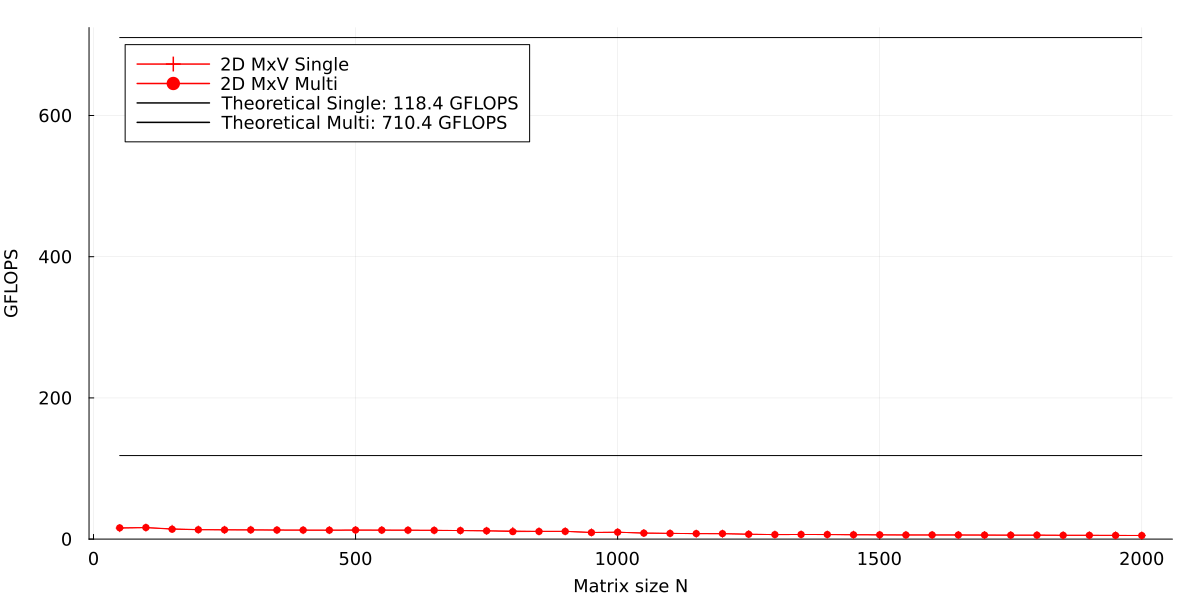
\includegraphics[width=\textwidth]{figures/8_wave_equation_solvers/Float32_GFLOPS_laplacian_2D_MxV.png}
\caption{\textbf{Float32 2D Laplacian (looped MxV): single vs. multi-threaded performance.} Both curves remain consistently low across all matrix sizes, with performance trapped in the 4-16 GFLOPS range. Single-threaded performance shows a declining trend with increasing size, while multi-threaded performance exhibits minimal improvement and similar degradation patterns.}
\end{figure}

\textbf{Consistently poor performance plateau}: Both curves remain trapped well below theoretical and practical performance levels achieved by other approaches, with performance ranging from 4-16 GFLOPS across all tested sizes. Unlike other implementations that show improvement or stability with increasing matrix size, both curves exhibit a general downward trend. Performance drops from peak values around 15-16 GFLOPS at small sizes to 4-6 GFLOPS for larger matrices.

\textbf{Threading ineffectiveness}: The \texttt{@threads} directive provides negligible performance improvements, with multi-threaded results closely tracking single-threaded performance throughout the tested range. This indicates that the explicit loop structure fundamentally limits effective parallelization, preventing the runtime from achieving meaningful speedups despite attempting thread-level parallelism.

This implementation validates the critical importance of algorithmic choice and library optimization, demonstrating that theoretical FLOP equivalence does not guarantee computational efficiency when implementation approaches differ fundamentally in their utilization of modern CPU architectures and optimized libraries.

\clearpage

\subsubsection*{2D Wave Equation (MxV Loop) FP64 Performance}

We evaluated the complete 2D wave equation solver across a range of grid sizes using \textbf{Float64 precision} and 1.0 second simulation time.

Each time step involves matrix-vector multiplication operations, plus additional operations for temporal integration and boundary condition enforcement. The total floating-point operations per time step can be approximated as $2 \times 2 \times N^3$ (dominated by the MxV operations):

\begin{equation}
\text{Total Operations} = \text{Time Steps} \times \text{Operations per Step} \approx N_t \times 2 \times 2 \times N^3
\end{equation}

We used an adaptive time step of $dt = 10^{-4} \times \frac{1}{N_{x}}$ seconds for stability control. This formulation ensures that finer grids use proportionally smaller time steps.

\vspace{1em}

\begin{tabular*}{\linewidth}{@{\extracolsep{\fill}}cccc}
\toprule
\textbf{Grid Size} & \textbf{Time (s)} & \textbf{Total Operations} & \textbf{GFLOPS} \\
\midrule
26 nodes  & 4.84   & 1.83 $\times$ 10$^{10}$ & 3.78 \\
51 nodes  & 30.64  & 2.71 $\times$ 10$^{11}$ & 8.83 \\
76 nodes  & 119.77 & 1.33 $\times$ 10$^{12}$ & 11.14 \\
101 nodes & 350.85 & 4.16 $\times$ 10$^{12}$ & 11.86 \\
126 nodes & 943.62 & 1.01 $\times$ 10$^{13}$ & 10.68 \\
\bottomrule
\end{tabular*}

\vspace{1em}

The performance progression demonstrates a different scaling behavior compared to the MxM implementation across all grid sizes. For small grids (26-51 nodes), we observe steady efficiency improvements as computational overhead is amortized. The medium to large grids (76-126 nodes) show peak performance around 10-11 GFLOPS, with a slight decline for the largest grid size.

This demonstrates the computational characteristics of 2D matrix-vector operations compared to matrix-matrix operations. While the total number of operations remains the same, the MxV implementation shows different performance characteristics due to memory access patterns and computational structure. The peak performance of approximately 11 GFLOPS is significantly lower than the 70 GFLOPS achieved in the MxM benchmark.

The performance plateau and slight decline for larger grids suggests that memory bandwidth limitations become more prominent in MxV operations, where the lower arithmetic intensity compared to MxM operations results in reduced computational throughput.

We observe that the MxV performance is substantially lower than what was achieved in the MxM benchmark, highlighting the importance of algorithmic choice and computational structure in high-performance computing applications, even when the total operation count remains constant.

\clearpage

\textbf{Physical 2D Wave Evolution (MxV) - Original Nodes Representation}

We see exactly the same physical wave evolution as in the matrix-matrix version.

The 2D solver captures complete wave physics on Chebyshev node grids. Using 25×25 nodes with 26-node stencils demonstrates radial wave propagation and boundary interactions:

\begin{figure}[H]
\centering
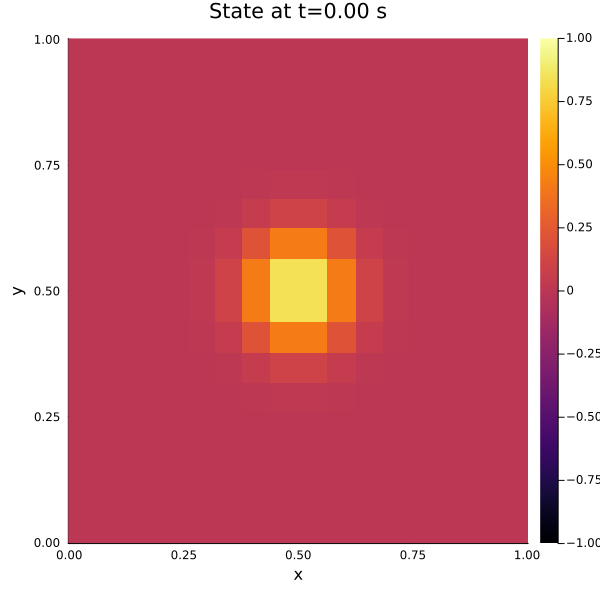
\includegraphics[width=0.48\textwidth]{code/8_wave_equation_solvers/benchmark_versions/output/output2D_25_MxV_benchmark/state_t_0.00.png}
\hfill
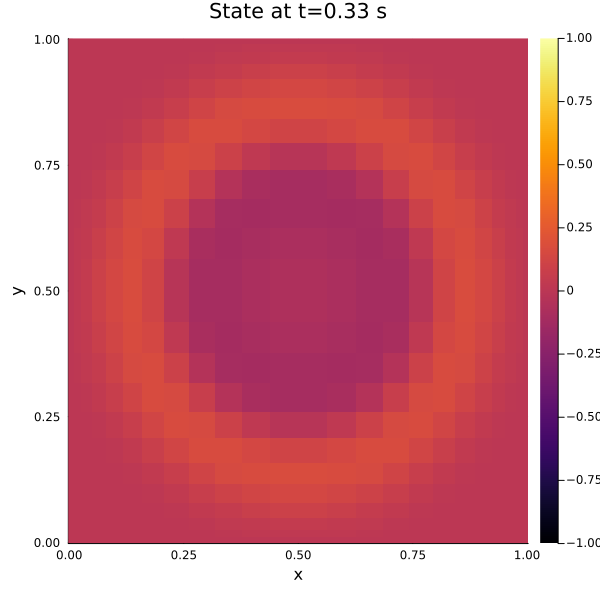
\includegraphics[width=0.48\textwidth]{code/8_wave_equation_solvers/benchmark_versions/output/output2D_25_MxV_benchmark/state_t_0.33.png}

\vspace{1em}

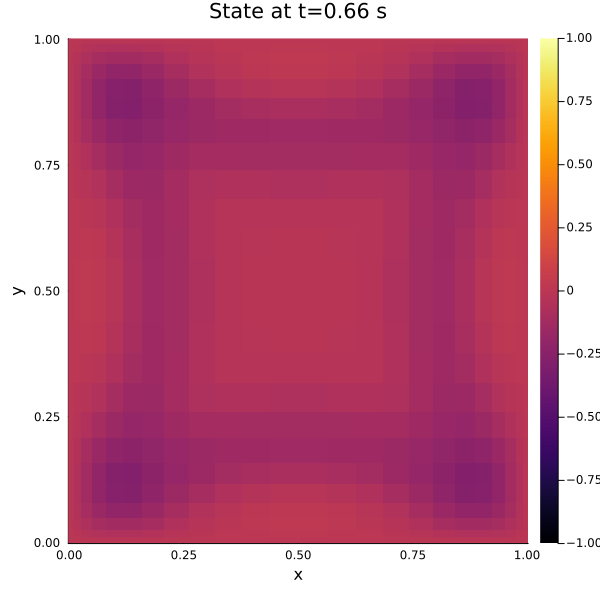
\includegraphics[width=0.48\textwidth]{code/8_wave_equation_solvers/benchmark_versions/output/output2D_25_MxV_benchmark/state_t_0.66.png}
\hfill
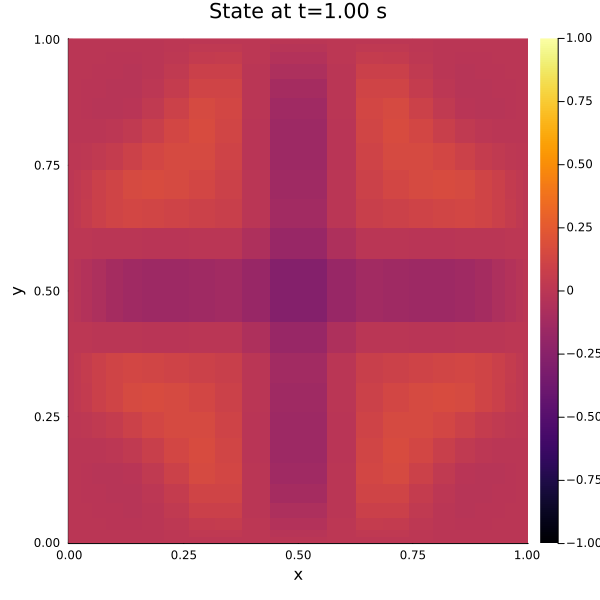
\includegraphics[width=0.48\textwidth]{code/8_wave_equation_solvers/benchmark_versions/output/output2D_25_MxV_benchmark/state_t_1.00.png}

\caption{\textbf{2D Wave Equation Evolution.} The temporal sequence shows: (top left) initial Gaussian pulse centered at domain center, (top right) radial wave expansion at t=0.33s, (bottom left) complex interference patterns at t=0.66s, and (bottom right) final standing wave configuration with multiple nodes at t=1.0s. The discrete solution is computed on a 26×26 Chebyshev node grid.}
\end{figure}

\clearpage

\textbf{Physical 2D Wave Evolution (MxV) - Interpolated Representation}

The 2D Chebyshev node distribution enables high-quality tensor-product Lagrange interpolation to reconstruct the continuous wave field. The solution is interpolated from 26×26 Chebyshev nodes to a 100×100 equispaced grid:

\begin{figure}[H]
\centering
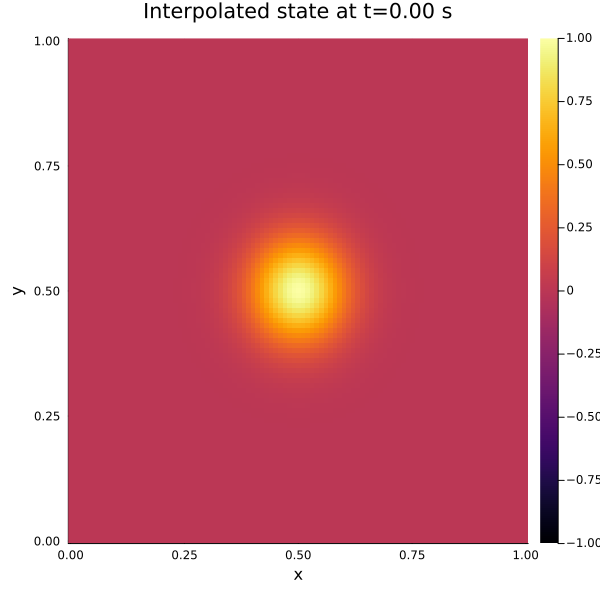
\includegraphics[width=0.48\textwidth]{code/8_wave_equation_solvers/benchmark_versions/output/output2D_25_MxV_benchmark/interpolated_state_t_0.00.png}
\hfill
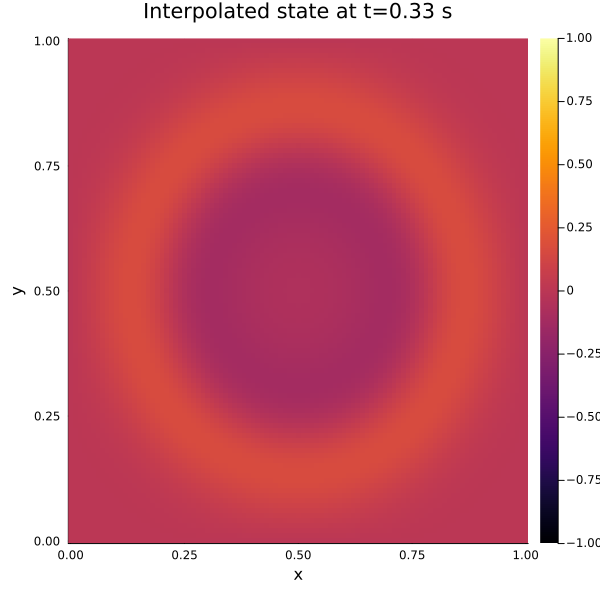
\includegraphics[width=0.48\textwidth]{code/8_wave_equation_solvers/benchmark_versions/output/output2D_25_MxV_benchmark/interpolated_state_t_0.33.png}

\vspace{1em}

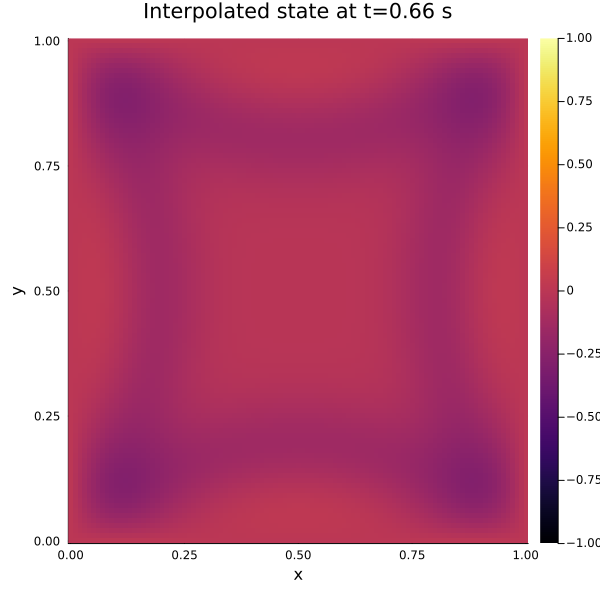
\includegraphics[width=0.48\textwidth]{code/8_wave_equation_solvers/benchmark_versions/output/output2D_25_MxV_benchmark/interpolated_state_t_0.66.png}
\hfill
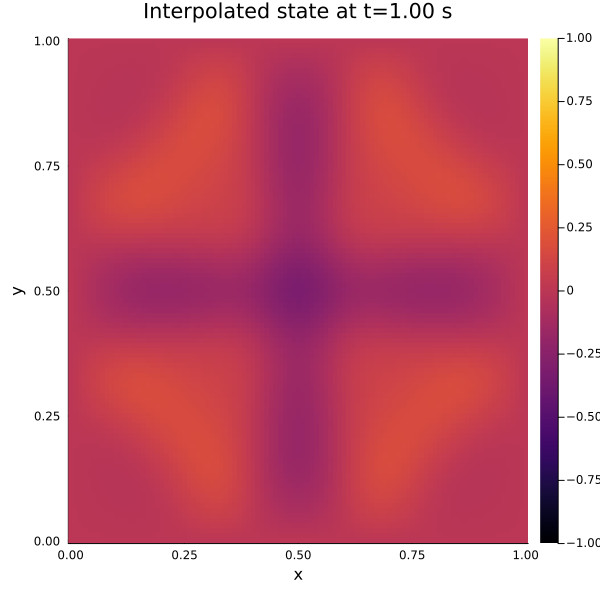
\includegraphics[width=0.48\textwidth]{code/8_wave_equation_solvers/benchmark_versions/output/output2D_25_MxV_benchmark/interpolated_state_t_1.00.png}

\caption{\textbf{2D Wave Equation Evolution (Fine Grid).} The smooth contours demonstrate excellent interpolation accuracy from the optimal 26×26 Chebyshev node distribution to a fine 100×100 equispaced visualization grid. The tensor-product interpolation preserves wave symmetry and captures fine-scale interference patterns throughout the temporal evolution.}
\end{figure}

\clearpage

\section{Wave Equation 2D in NumericalHub (Fortran)}
\label{sec:wave_2d_fortran}

\subsubsection*{2D Wave Equation NumericalHub (Fortran) Performance}

We evaluated the NumericalHub Fortran implementation of the complete 2D wave equation solver across a range of grid sizes using \textbf{Float64 precision} and 1.0 second simulation time. This serves as a benchmark comparison against our custom Julia implementations to assess the relative performance achieved by our developed codes.

The NumericalHub library uses established numerical methods with optimized Fortran implementations. Each time step involves the same fundamental operations as our implementations: spatial differentiation, temporal integration, and boundary condition enforcement. The total floating-point operations per time step follow the same approximation as $2 \times 2 \times N^3$:

\begin{equation}
\text{Total Operations} = \text{Time Steps} \times \text{Operations per Step} \approx N_t \times 2 \times 2 \times N^3
\end{equation}

The same adaptive time step formulation of $dt = 10^{-4} \times \frac{1}{N_{x}}$ seconds is used for stability control, ensuring consistent comparison conditions with our Julia implementations.

\vspace{1em}

\begin{tabular*}{\linewidth}{@{\extracolsep{\fill}}cccc}
\toprule
\textbf{Grid Size} & \textbf{Time (s)} & \textbf{Total Operations} & \textbf{GFLOPS} \\
\midrule
26 nodes & 12.06 & 1.56 $\times$ 10$^{10}$ & 1.29 \\
51 nodes & 228.03 & 2.50 $\times$ 10$^{11}$ & 1.10 \\
76 nodes & 792.80 & 1.27 $\times$ 10$^{12}$ & 1.60 \\
101 nodes & 1812.31 & 4.16 $\times$ 10$^{12}$ & 2.30 \\
\bottomrule
\end{tabular*}

\vspace{1em}

The NumericalHub Fortran implementation demonstrates consistent but modest performance across all grid sizes. Notably, this performance is significantly lower than both our Julia MxM implementation (which achieved up to 70 GFLOPS) and our Julia MxV implementation (which achieved up to 11 GFLOPS).

The comparison reveals several important insights about computational performance. While NumericalHub provides a robust, well-tested library solution, the performance characteristics suggest either more conservative algorithmic choices, additional computational overhead from generalized library functions, or different optimization strategies compared to our specialized implementations.

This performance comparison validates the effectiveness of our custom Julia implementations, demonstrating that targeted optimization and algorithmic design can achieve substantial performance improvements over general-purpose library solutions.

The consistent wave physics results across all implementations confirm that our optimized codes maintain numerical accuracy while delivering superior computational throughput.


\clearpage

\textbf{Physical 2D Wave Evolution (Fortran) Representation}

The 2D wave equation solver demonstrates complete wave physics on a 26×26 Chebyshev node grid. The implementation captures radial wave propagation from a central source and subsequent boundary interactions across the computational domain.

\begin{figure}[H]
\centering
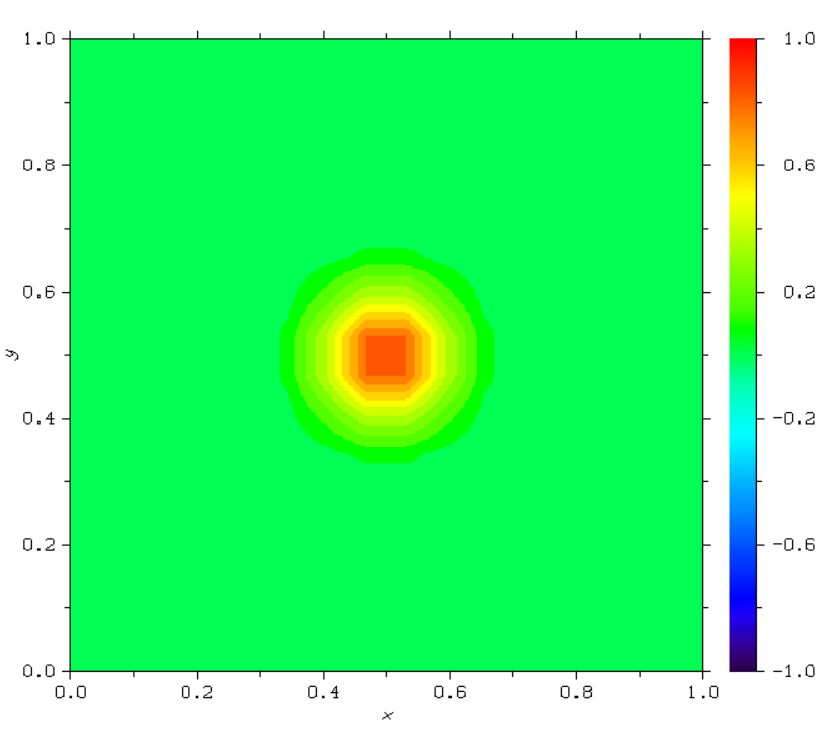
\includegraphics[width=0.48\textwidth]{code/8_wave_equation_solvers/benchmark_versions/output/fortran2D_benchmark/t0.0.png}
\hfill
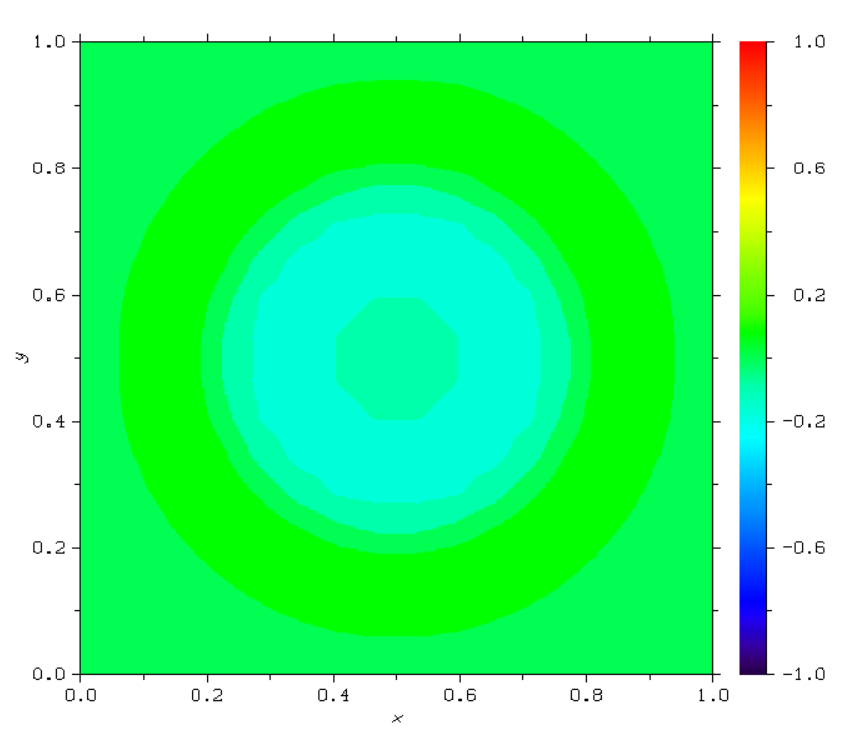
\includegraphics[width=0.48\textwidth]{code/8_wave_equation_solvers/benchmark_versions/output/fortran2D_benchmark/t0.33.png}

\vspace{1em}

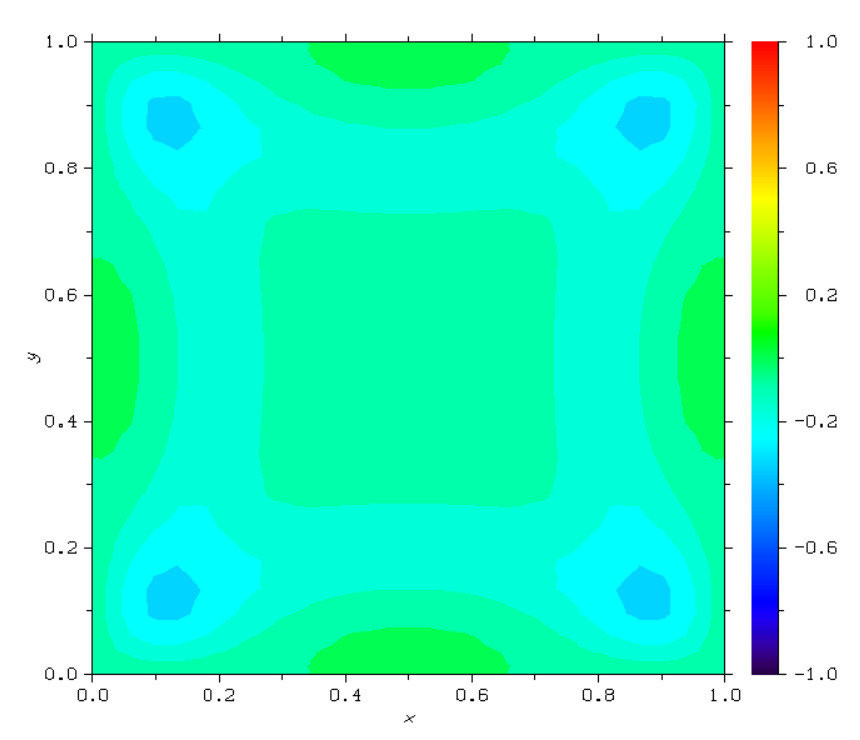
\includegraphics[width=0.48\textwidth]{code/8_wave_equation_solvers/benchmark_versions/output/fortran2D_benchmark/t0.66.png}
\hfill
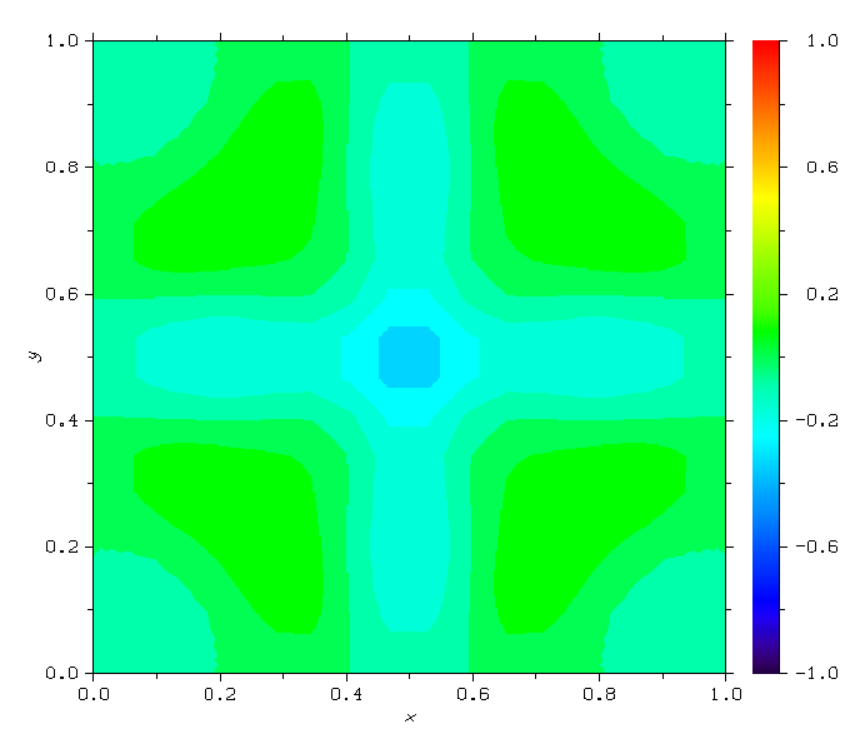
\includegraphics[width=0.48\textwidth]{code/8_wave_equation_solvers/benchmark_versions/output/fortran2D_benchmark/t1.0.png}

\caption{\textbf{2D Wave Equation Evolution.} Numerical solution of the 2D wave equation implemented in NumericalHub and visualized using the plot\_contour function.}
\end{figure}

This visualization represents the same numerical approach implemented in the Julia versions, but executed through the NumericalHub framework with Dislin-based contour plotting for scientific visualization.


